\documentclass{article}
\usepackage[margin=1.25in]{geometry}
\usepackage{amsmath, amssymb, setspace, enumerate, enumitem}
\usepackage{setspace}
\usepackage{graphicx}
\onehalfspacing

\begin{document}
    \begin{enumerate}
        \item Exercise 2.4
        \begin{enumerate}
            \item Consider the following matrix:\\
            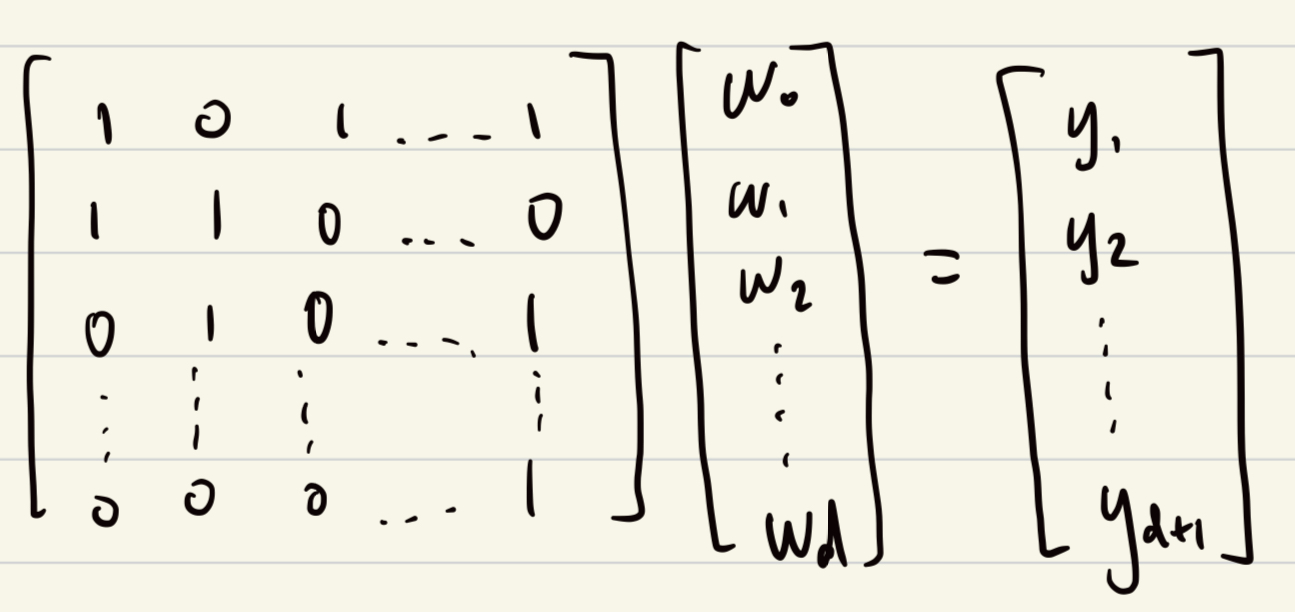
\includegraphics[scale=0.25]{img/2_4.jpeg}\\
            Since this is a non-singular matrix, we know that every system $Ax = b$ has a unique solution, if we are able to find a hypothesis with weights w such to produce our solution $y$, then it is true that there exist at least one hypothesis that can shatter those points.
            
            \item For $d+2$ points, where each point has dimension $d + 1$, any $d + 2$ vetors of length $d + 1$ has to be linearly dependent.\\
            However, intuitively, it's possible to have less poitns than dimensions in a linear independent set, but if we have more points than dimensions, it is no possible, which is the case that we have.\\
            Consider our $d + 2$ vector, $x_{d+2}$, where $x_{d+2} = \sum_{i = 0}^{d + 1} c_ix_i$, if we have a dichotomy where $w^Tx_nc_n <0$ for each point n, assuming that the dichotomy holds for $d+2$ points, then $sign(w^Tx_{d+2}) = -1$, a situation where the positive dichotomy cannot be implemented. (a) and (b) proves that the VC dimension of the perceptron is exactly $d+1 \hfill \blacksquare$
        \end{enumerate}

        \item Problem 2.3
        \begin{enumerate}
            \item Consider example 2.2 (i):\\
            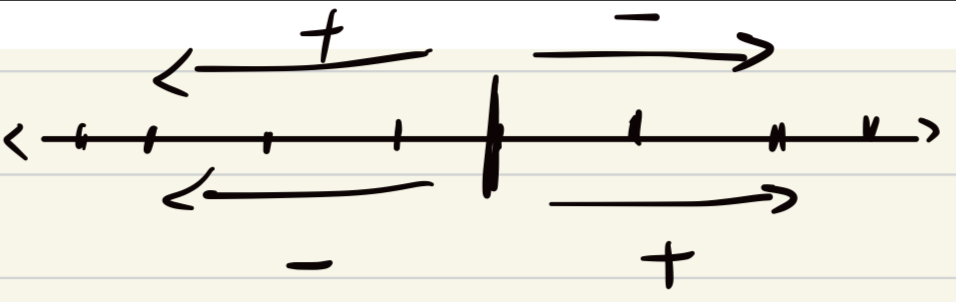
\includegraphics[scale=0.25]{img/2_3_1.jpeg}\\
            We can split the line in $N+1$ different places, each place has two possible rays, so we construct $2(N+1)$.\\
            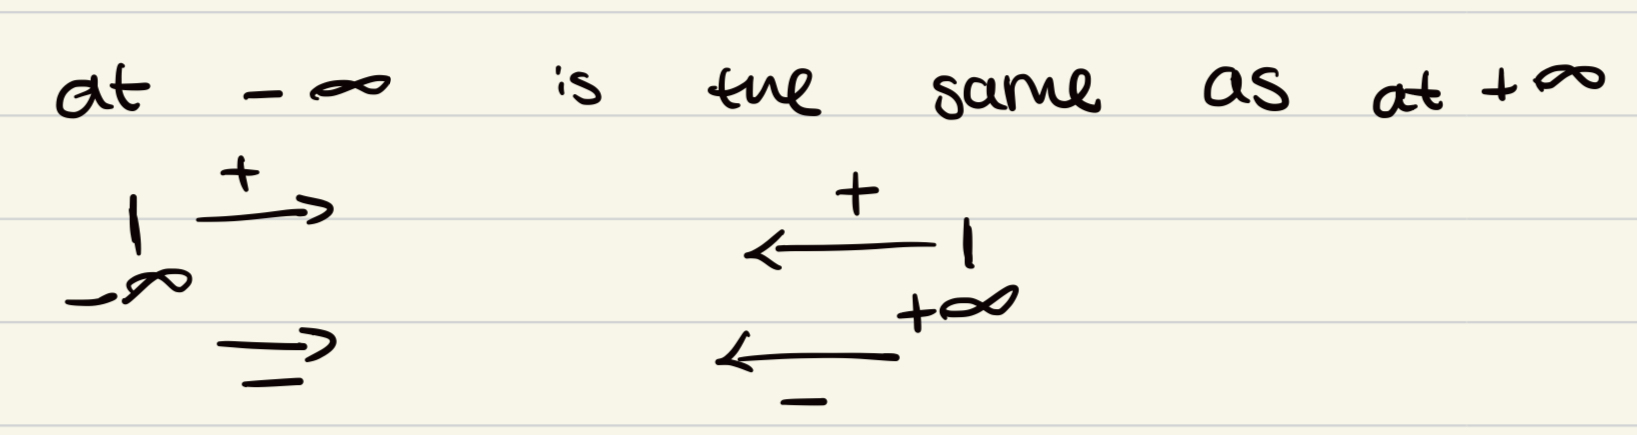
\includegraphics[scale=0.15]{img/2_3_2.jpeg}\\
            So $m_H(N) = 2N + 2 - 2 = 2N$\\
            For $k = 2$: $2^2 = 4 \rightarrow 2(2) = 4$\\
            For $k = 3$: $2^3 = 8 \rightarrow 2(3) = 6$\\
            So breakpoint at $k = 3$, so $d_{vc} = k - 1 = 2$

            \item Consider example 2.2 (ii):\\
            In the case where it is only a positive interval, we have $\frac{1}{2}N^2 + \frac{1}{2}N + 1$, counting positive and negatives, we can multiply it by 2, giving us $N^2 + N + 2$.\\
            Range of $[-\infty, a]$ being positive is the same as $[a, \infty]$ being negative, and vise versa, this applies for all $a \in N$, so we can remove $2N$, giving us the following equation $N^2 - N + 2$.\\
            $k = 2$, we have $2^2-2+2=4=2^2$\\
            $k = 3$, $3^2-3+2=8=2^3$\\
            $k = 4$, $4^w-4+2=14\neq 2^4$, so our breakpoint is at $k = 4$, $d_{vc} = k - 1 = 3$

            \item Consider example 2.2 (ii):\\
            We can use the positive interval example to bond a concentric sphere in $d$ dimensions similarly. From hw3, exercise 2.3 part(2), this concentric sphere is in $d_{vc} = 2$ since it has a breakpoint at $k = 3$.
        \end{enumerate}

        \item Problem 2.8\\
        From lecture (6), possible growth functions are either $2^N$ or $\exists$ a breakpoint $k$ such that $m_H(N) \leq N^{k-1} + 1$.
        \begin{enumerate}[label=(\roman*)]
            \item Yes, $1 + N$, by inspection, breakpoint at $N=2$, so $m_H(3) \leq 3 + 1$ where $m_H(3) = 4$, so it is valid, $m_H(N) = N + 1$, $N^{2-1} + 1 = N +1$
            \item Yes, $1 + N + \frac{N(N-1)}{2}$, at $N =3$, then it equals $7$, $7 < 2^3$, so $k = 3$ is our breakpoint. $1 + N + \frac{N^2 - N}{2} = \frac{N^2}{2} + \frac{N}{2} + 1 \leq N^2 + 1$, by inspection, we see that it grows slower than $N^2 + 1$ since it is being divided by 2, therefore it is corect.
            \item Yes, $2^N$ is a power of 2, so it is valid.
            \item No, for $N=2$, $2^{f\ \sqrt{2}} = 2 < 2^2$ (I don't know how to do floor symbol on latex, assume f = floor), therefore $k = 2$ is a breakpoint, so $2^{f \sqrt{N}} \leq N + 1$, we can see this is not true by inspection, since for $N = 100$, $2^{10} \nleq 101$.
            \item No, $2^{f\frac{N}{2}}$, $k = 2$ by inspection is our breakpoint, choose a high $N$, we can see that $2^{f\frac{N}{2}} \nleq N + 1$, same reasoning as (iv).
            \item No, for $k = 2$, the equation evaluates to $3 < 2^2$, so it is our breakpoint. this means that $1 + N + \frac{N(N-1)(N-2)}{6} < N + 1$, if we try $ N = 10$: $11 + \frac{10(9)(8)}{6} = 11 + 5 \times 3 \times 8 = 131 \nleq 11$
        \end{enumerate}

        \item Problem 2.10\\
        Consider $D$ and $D^\prime$ where $D$ and $N$ datapoints and $D^\prime$ has $N$ datapoints as well, but $D$ and $D^\prime$ contain completely different datasets. We can take any dichotomy in $D$ and match it with all the dichotomies in $D^\prime$, creating one dichotomy of $2N$ points. If you take all the dichotomies and match them respecitvely, you will get at most $m_H(N)^2$ dichotomies, which is where we receive the upperbound, therefore $m_H(2N) \leq m_H(N)^2$, hence we can change our vc generalization bound from $E_{out} \leq E_{in} + \sqrt{\frac{8}{N}\ln{\frac{4m_H(2N)}{\delta}}}$ to $E_{out} \leq E_{in} + \sqrt{\frac{8}{N}\ln{\frac{4m_H(N)^2}{\delta}}}$.

        \item Problem 2.12\\
        From (2.13)
        \begin{align*}
            N \geq \frac{8}{\epsilon^2}\ln{\frac{4((2N)^{d_{vc}}+1)}{\delta}}
        \end{align*}
        We need $95\%$ confidence, so $\delta = 0.05$, we need generalization error at most $0.05$, so $\epsilon = 0.05$, so
        \begin{align*}
            N \geq \frac{8}{0.05^2}\ln{\frac{4((2N)^{10}+1)}{0.05}}
        \end{align*}

        From example 2.6, we continue to guess and iterate: $d_{vc} = 10$, we can try $N = 10000$

        \begin{align*}
            N \geq \frac{8}{0.05^2}\ln{\frac{4((2(10000))^{10}+1)}{0.05}} &= 330934\\
            N \geq \frac{8}{0.05^2}\ln{\frac{4((2(330934))^{10}+1)}{0.05}} &= 442912\\
            N \geq \frac{8}{0.05^2}\ln{\frac{4((2(442912))^{10}+1)}{0.05}} &= 452239\\
            N \geq \frac{8}{0.05^2}\ln{\frac{4((2(452239))^{10}+1)}{0.05}} &= 452906\\
        \end{align*}

        Appears to converge somewhere close to $452906$, so we can say that $N \geq 452906$.
    \end{enumerate}
\end{document}

